%%
%z = FF+M
%kr = k*W/w
%%
%one = ( (z*(z+k))/(alpha*w*(z+kr)) )^gamma
%two = (gamma*FF/alpha/w) * ((z*(z+k))/(alpha*w*(z+kr)))^(gamma-1)
%thr = kr*(k-kr)/((z+kr)^2)
%
\newcommand{\kr}{ \frac{\kappa w_\infty}{w(a_s)} }
\newcommand{\one}{
        \left(\frac{Z(Z+\kappa)}{\alpha w(a_s)(Z+\kr)}\right)^\gamma
}
\newcommand{\two}{
        \left(\frac{\gamma F}{\alpha w(a_s)}\right) \left(\frac{Z(Z+\kappa)}{\alpha w(a_s)(Z+\kr)}\right)^{\gamma-1}
}
\newcommand{\thr}{
        \frac{\left(\kr\right)\left(\kappa-\kr\right)}{(Z+\kr)^2}
}
%
\newcommand{\oneA}{
        \left(\frac{Z^*(Z^*+\kappa)}{w(a_s)(Z^*+\kr)}\right)^\gamma
}
\newcommand{\twoA}{
        \left(\frac{\gamma F^*}{w(a_s)}\right) \left(\frac{Z^*(Z^*+\kappa)}{w(a_s)(Z^*+\kr)}\right)^{\gamma-1}
}
\newcommand{\thrA}{
        \frac{\left(\kr\right)\left(\kappa-\kr\right)}{(Z^*+\kr)^2}
}



%
\section{Introduction}

%
\begin{itemize}
\item the delay model: \cite{schnute_general_1985} \cite{schnute_general_1987} \cite{fournier_length-based_1987}.
\item discrete: \cite[pg. 334]{hilborn_quantitative_1992}
\item \cite{walters_continuous_2020}
\item automatic accounting for cohort cycles
\end{itemize}

%
\section{Methods}

%
\subsection{Delay Differential Model}

%
\begin{wrapfigure}{r}{0.45\textwidth} %[17]{r}[0pt]{0pt}%
%\begin{figure}[h!]
\vspace{-1cm}
%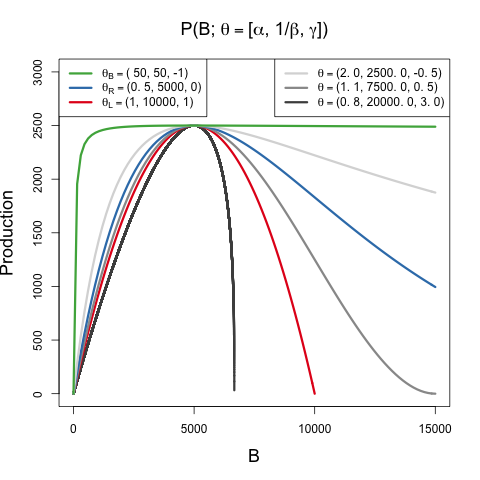
\includegraphics[width=0.5\textwidth]{plots/derisoSrr.png}
%\begin{minipage}[h!]{0.64\textwidth}
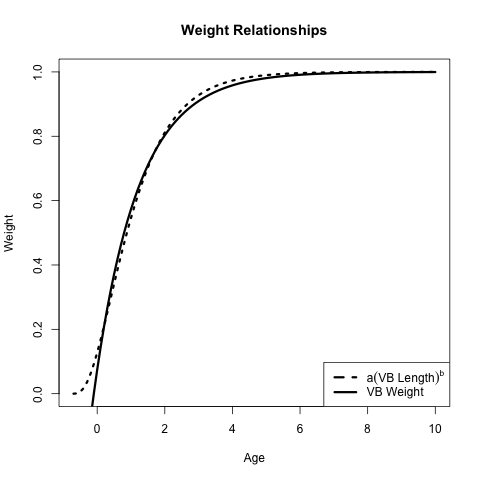
\includegraphics[width=0.49\textwidth]{plots/vbOpt.png}
%\end{minipage}
%\begin{minipage}[h!]{0.3\textwidth}
\vspace{-1cm}
%\hspace*{-1cm}
\caption{
%\onehalfspacing
The typical composition of allometric weight ($b=3$) with VB growth in length, as
approximated by VB growth in weight directly.
%A comparison of 
%with the typical assumption of VB growth in length. 
}
\label{SrrPT}
%\end{minipage}
\end{wrapfigure}

%
Age structured fisheries models typically assume %Von Bertalanffy (VB) growth 
\cite[VB]{von_bertalanffy_quantitative_1938} gorwth in length with age. To model
weight the assumption of VB growth in length is composed with a power law 
relating length to weight, $w=al^b$. 
%The statistical model then assumes observed indicies of abundance are proportional to weight. 
%
Since $b$ is usually $\sim3$ this composition of assumed functional forms
typically results in a monotonically increasing sigmoidal curve of weight with age.
When $b\le1$ weight at age takes a VB-like form with $b=1$ resulting in
an exact correspondence of simulanious VB-growth in length and weight.

%
The delay model slightly abridges these relationships by directly assuming VB
growth in weight as follows,
%%
%\begin{align}
%\frac{dw}{da} &= \kappa(w_\infty-w(a)) \label{wODE}
%\end{align}
%
\begin{align}
w(a) &= w_\infty(1-e^{-\kappa (a-a_0)}). \label{vbGrowth}
\end{align}
%
$\kappa$ is a parameter that controls the instantaneous rate of individual
growth (in weight) with age. $w_\infty$ is the maximum weight of individuals
in the population, and $w(a)$ is the average weight of an individual at
age $a$. The parameter $a_0$ controls the age at which individuals are assummed
to have zero weight; by letting $a_0<0$ this allows fish of age zero to have
positive weight. Rather than taking a sigmoidally increasing function, VB growth
directly in weight results in an monotonically inceasing curve that asymptotes
with a strictly decreasing growth rate with age.
{\color{red}(only a good approximation for older ages where growth begins to decline)}

%
Together with VB growth, the delay model is derived from the assumption that
both natural mortality and fishing selectivity are separately propotional
%the total mortality rate (from both natural and fishing mortality) is proportional 
to a common heavyside step function with age. That is to say, before a threshold
age of selectivity, $a_s$, the population is assumed not to experience any
mortality whatsoever, but all fish older then $a_s$ experience the same rate
of natural mortaility. Simulaneously all fish older than $a_s$ are equally
vulnerable to fishing (i.e. knife edge selectivity at age $a_s$), although
fishing effort may vary from through time.

%
\cite{walters_continuous_2020} shows that within these assumptions the
following delay differential system of equations exactly models the population
dynamics of the total exploitable biomass $B(t)$ and number of indivuduals $N(t)$
through time.
%%
%\begin{align}
%B(t) = \int^\infty_{a_s} N(a, t)w(a) da
%\end{align}
%
\begin{align}%\kappa->0 slower than a0->\infty
%B(a, t) &= w(a, t)N(a, t)\\ 
%\frac{dB}{dt} &= \overbrace{w(k)R(B(t-k))}^\text{Recruitment Biomass} + \overbrace{\mu w_\infty N(t)}^\text{Growth} - \overbrace{(M+F(t)+\mu)B(t)}^\text{Biomass Loss}\\
&\frac{dB}{dt} = w(a_s)R(B;\theta) + \kappa \left[w_\infty N-B\right] - (M+F)B \label{bEq}\\
&\frac{dN}{dt} = R(B;\theta) - (M+F)N \label{nEq}
%&R(B;[\alpha, \beta, \gamma]) = \alpha B(t-a_s)(1-\beta\gamma B(t-a_s))^{\frac{1}{\gamma}} \label{srr}\\
%&w(a) = w_\infty(1-e^{-\kappa a}) \label{vbGrowth}
\end{align}

%
This formulation separates the number of individuals in the population from the
biomass of the population. The dynamics of $N$, as seen in Eq (\ref{nEq}), are
very similar to that of the {\color{green}production models previously presented}, 
however the role of the production function is now filled by a "recruitment"
function, $R(B)$, which describes the number of new individuals recruiting into the
expoitable population as a function of exploitable biomass. In turn, the biomass
dynamics are coupled to the numbers dynamics by the assumption of VB growth with
growth parameters appearing in Eq (\ref{bEq}), converting population numbers
into biomass and accounting for the growth of biomass with age.

%
Eq (\ref{bEq}) of the above model expands the notion of biomass production into the
processes of recruitment, individual growth, and maturity. The term $w(a_s)R(B;\theta)$
represents the biomass of new recruits; with $w(a_s)$ representing the weight of individuals
at the age of maturity, $a_s$, and $R(B;\theta)$ representing the number of new recruits
entering the exploitable population at time $t$. The negative term, $(M+F)B$, represents all
causes of mortality as it is applied to biomass. Finally, the term $\kappa \left[w_\infty N-B\right]$
accounts for the net growth of the existing biomass by discounting the limiting maximal individual
growth rate by metabolic weight loss proportional to $B(t)$. This term, together with the delay
structure in $R$, provides the major computational savings of the delay differential setting, as
compared with full age structured models, by automatically keeping track of changes in the mean
size and growth associated with changes in recruitment as cohorts mature into the population.
%The framework is likely to perform very well at this task, considering that growth and natural 
%survival rates tend to be fairly stable over time in fishes.

%
Often a BH functional form is assumed for the stock recruitment relationship, but any adequatly
flexible family of functions may model this relationship. For the sake of evaluating the adequacy
of assumed BH recruitment the simulation setting below is derived for the delay model under the
assumption of the generalized three parameter Schnute recruitment as follows.
%
\begin{align}
R(B;[\alpha, \beta, \gamma]') = \alpha B(t-a_s)(1-\beta\gamma B(t-a_s))^{\frac{1}{\gamma}} \label{srr}
\end{align}
%
The parameters $\bm{\theta}'=[\alpha, \beta, \gamma]$ %\alpha$, $\beta$, and $\gamma$, 
function similarly in this setting as previously described in Section (\ref{}).
That said, since the delay model explicitly parses out growth in it's dynamics,
these parameters only describe the net processes of larval production, and maturation
into the population, where as the production model used these parameters to
also model the net effects of growth on biomass production. %NOTE: production model includes net growth in in the nonlinear form of P, while the delay model used VB Growth params (functional form) on top of this nonlinearity. 
The $\gamma$ parameter generalizes the family to model varying degrees of
decreasing recruitment for large biomasses as $\gamma$ increases. The Schnute
function is exactly equivalent to BH recruitment at the special case when
$\gamma=-1$, it passes through the Ricker model as $\gamma\rightarrow0$, and
Logistic recruitment occurs when $\gamma=1$.

%%the exploitable biomass of the population becomes large
% controls the behavior of recruitment from the special case of BH recruitment at $\gamma=-1$, 
%The structure of the Schnute function here is similar to that of the previously described, with $\gamma$ . 
%
Since the delay model assumes knife edge selectivity, at age $a_s$, the term
$B(t-a_s)$ appears in $R$. That is to say fish recruiting into the exploitable
population are the result of larval production of biomass $a_s$ time
units in the past. This is because fishing selectivity is only assumed to occur
for fish that are at least $a_s$ time units old and thus fish younger than $a_s$
are not exploitable. This waiting period requires that new recruits be the
result of spawning biomass $a_s$ time units in the past. Modeling maturity in
this way results in dynamics equations which are a system of delay differential
equations as opposed to the simple ODEs that arrise in the production model
setting.
%which is where the delay differential equation  

%
\begin{itemize}
        %\item parameters $\alpha$, $\beta$, and $\gamma$,
        %\item The BH and Logistic production functions arise when $\gamma$ is fixed to -1 or 1 respectively. 
        %\item The Ricker model is a limiting case as $\gamma\rightarrow0$. %\shortcite{schnute_general_1985}.
        %\item For $\gamma<-1$ a family of strictly increasing Cushing-like curves arise,
        %       culminating in linear production as $\gamma\to-\infty$. These special cases form
        %       natural regimes of similarly behaving production functions as seen in Figure (\ref{sRegimes}).
        %\item time delay
        \item[$\sim$] interpretation of recruitment (larval production, recruitment) [growth external] vs. production (larval production, recruitment, growth)
\end{itemize}

\begin{itemize}
\item general structure: \cite{walters_continuous_2020} \cite[pg. 334]{hilborn_quantitative_1992}
\item growth: \cite{von_bertalanffy_quantitative_1938}
\item recruitment: \cite{schnute_general_1985, schnute_analytical_1998}
\end{itemize}


%
\subsection{Reference Points}

%
Deriving reference points for the delay model under Schnute recruitment is
conceptually similar to the production model setting. The additional nonlinear
VB growth assumptions along side Schnute recruitment quickly make the
expressions look somewhat unweildy, although analytical solutions can still be
derived for most of the same quantities (although complicated by growth parameters).

%
Starting from Eqs. (\ref{bEq}) and (\ref{nEq}), setting both $\frac{dB}{dt}$
and $\frac{dN}{dt}$ simultaneously equal to zero, and solving for $B$ and $N$
as a function of fishing, gives the equilibrium biomass and numbers equations.
%
\begin{align}
\bar{B}(F) &= \frac{1}{\beta\gamma} \left( 1 - \Big(\frac{(F + M) (F + M + \kappa)}{\alpha w(a_s)(F + M + \kr)}\Big)^\gamma\right) \label{BF}\\
%\end{align}
%\begin{align}
\bar{N}(F) &= \frac{\alpha\bar{B}(F)(1-\beta\gamma\bar{B}(F))^{1/\gamma}}{F+M} \label{NF}
\end{align}
%
Eq. (\ref{NF}) is just $\frac{R(\bar{B})}{F+M}$, and is coupled to $\bar{B}(F)$
where most of the dynamics appear. Eq. (\ref{BF}) resembles Eq (\ref{BsEq})
from the simple production model setting although the growth parameters
$\kappa$, $w_\infty$ and $w(a_s)$, make slight adjustments to the balance of the
maximum rate of recruitment and mortaility rate to give an expression for
equilibrium biomass that accounts for the factors of individual growth.
% for the produce to a more complex expression for equilibirum biomass.

%
Expressions for $B_0$ and $B^*$ are attained by evaluating $\bar{B}(F)$ at
$F=0$ and $F=F^*$ respectively. Calculation of $F^*$ typically involves %amounts to %requires %Obtaining an expression for 
maximization of equilibrium yield, \mbox{$\bar{Y} = F\bar{B}(F)$.} While it was not
possible to analytically maximize $\bar{Y}$, stable numerical solutions for
calculating $F^*$ were obtained by numerically solving for the roots of the
analytical derivative of equilibrium yield with respect to $F$. Below a greatly
simplifed expression for $\frac{d \bar{Y}}{dF}$ is shown; the substitution
$Z=F+M$ (total mortality rate) has been made to produce a more compact expression.

%
\vspace{-0.75cm}
\begingroup
\scriptsize
\begin{align}
\frac{d \bar{Y}}{dF} &= \frac{1}{\beta\gamma}\left[ 1 - \one - \two \left( 1 + \thr \right) \right]\label{dBdFS}
%&= (1-\left(\frac{(F+M)*(F+M+\kappa)}{\alpha*(F*w(a_s)+M*w(a_s)+\kappa*w_infty)}\right)^\gamma-(F*(((F+M)*(F+M+\kappa))/(\alpha*(F*w(a_s)+M*w(a_s)+\kappa*w_infty)))^(\gamma-1)*\gamma*(\alpha*(F*w(a_s)+M*w(a_s)+\kappa*w_infty)*(2(F+M)+\kappa)-(F+M)*(F+M+\kappa)*\alpha*w(a_s)))/(\alpha*(F*w(a_s)+M*w(a_s)+k*w_infty))^2)/(\beta\gamma) \label{dBdFS}.
%&= ( 1-\Big(\frac{(F+M)(F+M+\kappa)}{\alpha w(a_s)(F+M+\kappa w_\infty/w(a_s))}\Big)^\gamma - ( F*( ((F+M)*(F+M+\kappa))/(\alpha*(F*w(a_s)+M*w(a_s)+\kappa*w_infty)) )^(\gamma-1)*\gamma*(\alpha*(F*w(a_s)+M*w(a_s)+\kappa*w_infty)*(2(F+M)+\kappa)-(F+M)*(F+M+\kappa)*\alpha*w(a_s)) )/( \alpha*(F*w(a_s)+M*w(a_s)+k*w_infty))^2)/(\beta\gamma) \\
\end{align}
\endgroup
%
$F^*$ is calculated as the numerical root, w.r.t. $F$, of the above expression.
The numerical root is calculated using the base R uniroot function which
employs a derivative free search given by \cite{brent_chapter_1973}. %\shortciteA{brent_chapter_1973}.

%
\subsubsection{BH Constraint}

%
\begin{wrapfigure}{r}{0.50\textwidth} %[17]{r}[0pt]{0pt}%
%\begin{figure}[h!]
\vspace{-2.75cm}
%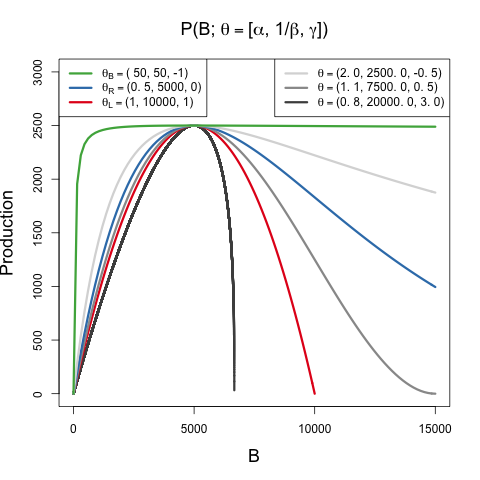
\includegraphics[width=0.5\textwidth]{plots/derisoSrr.png}
%\begin{minipage}[h!]{0.64\textwidth}
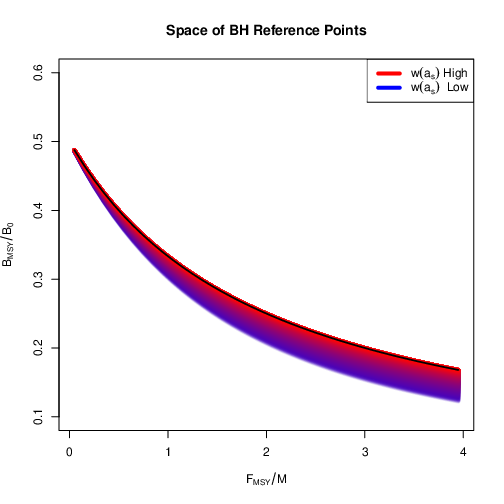
\includegraphics[width=0.54\textwidth]{../ddBias/rpSpaceww.png}
%\end{minipage}
%\begin{minipage}[h!]{0.3\textwidth}
\vspace{-1.5cm}
%\hspace*{-1cm}
\caption{
\onehalfspacing
The space of BH RPs for the delay model as a function of $\kappa$ and $a_s$.
The RP space is plotted for $80\times80$ combinations of $\kappa\in[0.1, 2]$
and $a_s\in[0.1, 10]$. The color drawn is the resulting value of $w(a_s)$
mapped between blue and red.
%the result of mapping $\kappa$ and $a_s$ values to the red and blue components of the RGB color model repsectively (with G=0). 
$\frac{1}{x+2}$ is plotted in black for reference.
%
}
\label{rpSpace}
%\end{minipage}
\end{wrapfigure}
%\end{figure}



